\chapter{Toroidal graphs}

Recall that a graph is called \index{planar graph}\emph{planar} if it can be drawn on a plane with no crossings; the latter is equivalent to existence of its drawing on a sphere.
Here and further, we say \index{drawing}\emph{drawing} for \emph{drawing with no crossings}.  

\begin{wrapfigure}{o}{40 mm}
\vskip-2mm
\centering
\includegraphics{mppics/pic-101}
\end{wrapfigure}

In this chapter we will discuss drawing of graphs on a torus --- another surface that can be obtained by revolving a circle about an axis (this is the surface of a donut).

A graph is called \index{toroidal graph}\emph{toroidal}, if it can be drawn on a torus with no crossing.

If one cuts a torus along a parallel and a meridian as shown on the diagram,
then the obtained surface can be developed into a square.%
\footnote{Formally speaking it means that there is a continuous map $f\:\square\to T$ from a square to torus  such that $f(x)=f(y)$ if and only if $x=y$ or $x$ and $y$ are corresponding points on the opposite sides of the square.}
It gives a convenient way to describe drawings of graphs on the torus which will be called \index{square diagram}\emph{square diagram}.
One only has to remember that the corresponding points on the opposite sides of the square are identified in the torus;
in particular all four vertexes of the square correspond to one point in the torus.

{

\begin{wrapfigure}{r}{30 mm}
\vskip-4mm
\centering
\includegraphics{mppics/pic-102}
\end{wrapfigure}

For example, on the given square diagram you see a drawing of the  complete graph $K_5$;
in particular it shows that $K_5$ is toroidal.
Note that the edge $xy$,
after coming to the right side of the square, reapers at the corresponding point of the left side and goes further to~$y$.
Similarly, the edge $vw$ comes to the top and reapears at the botom.
At these points on the edges cross the parallel and the meridian.

}

The following square diagrams show that $K_{4,4}$ and $K_7$ are toroidal graphs as well.

\begin{figure}[h!]
\begin{minipage}{.48\textwidth}
\centering
\includegraphics{mppics/pic-104}
\end{minipage}\hfill
\begin{minipage}{.48\textwidth}
\centering
\includegraphics{mppics/pic-106}\label{K5-toroidal}
\end{minipage}

\medskip

\begin{minipage}{.45\textwidth}
\centering
\caption*{$K_{4,4}$}
\end{minipage}\hfill
\begin{minipage}{.45\textwidth}
\centering
\caption*{$K_7$}
\end{minipage}
\vskip-4mm
\end{figure}




\begin{thm}{Exercise}
Show that any graph with crossing number 1 is toroidal.
That is, if a graph admits a drawing on a sphere with one crossing, then it admits a drawing on a torus with no crossings.
\end{thm}


\begin{thm}{Exercise}
Show that each of the following graphs is toroidal; construct a corresponding square diagram in each case.

(a) \includegraphics{mppics/pic-107}
(b) \includegraphics{mppics/pic-108}
(c) \includegraphics{mppics/pic-117}
\end{thm}


\section*{Simple regions}

Choose a drawing $G$ of a pseudograph on a torus or sphere;
it subdivides the the surface into regions.
A region $R$ is called \index{simple region}\emph{simple} if its interior can be parameterized by an open plane disc.%
\footnote{Formally speaking it means that the there is a continuous bijection from interior of $R$ to an open disc in the plane such that its inverse is also continuous.}

\begin{wrapfigure}{r}{30 mm}
\vskip-4mm
\centering
\includegraphics{mppics/pic-109}
\end{wrapfigure}

The annulus shown the diagram is an example of a nonsimple region.
On a sphere it may appear only in drawings of nonconnected graphs.
That is, if a drawing of a pseudograph $G$ on a sphere has a nonsimple region, then $G$ is not connected.
This statement should be intuitively obvious, but the proof is not trivial.  

Drawings of connected graphs on torus may have nonsimple regions.
For example, in the first drawing of $K_4$ below,
\begin{figure}[h!]
\begin{minipage}{.45\textwidth}
\centering
\includegraphics{mppics/pic-110}
\end{minipage}
\hfill
\begin{minipage}{.45\textwidth}
\centering
\includegraphics{mppics/pic-111}
\end{minipage}

\medskip

\begin{minipage}{.45\textwidth}
\centering
\caption*{$p=4$, $q=6$, $r=3$; the regions $B$, $C$ are simple, and $A$ is not.}
\end{minipage}\hfill
\begin{minipage}{.45\textwidth}
\centering
\caption*{$p=4$, $q=6$, $r=2$; both regions $D$ and $E$ are simple.}
\end{minipage}
\vskip-4mm
\end{figure} 
the regions $B$ and $C$ are simple and the region $A$ is not (it contains the meridian of the torus).
The second drawing of $K_4$ has only two regions $D$ and $E$ and both of them are simple.


Further we will use the following claim which should be intuitively obvious.
We do not present its proof, but it is not hard;
a reader familiar with topology may consider it as an exercise.

{

\begin{wrapfigure}{r}{15 mm}
\vskip-4mm
\centering
\includegraphics{mppics/pic-121}
\medskip
\includegraphics{mppics/pic-120}
\end{wrapfigure}

\begin{thm}{Claim}\label{clm:cut}
Let $G$ be a drawing of a pseudograph on a torus or sphere and $R$ its simple region.
Suppose that a drawing $G'$ obtained from $G$ by adding a new edge $e$ in the region $R$.
\begin{enumerate}[(a)]
\item If both of vertexes of $e$ are in $G$ (the edge $e$ might be a loop), then $e$ divides $R$ into two simple regions.
\item If only one of vertexes of $e$ are in $G$, then $e$ does not divide $R$ and the corresponding region of $G'$ is simple.
\end{enumerate}
\end{thm}

}

\begin{thm}{Advanced exercise}
Suppose that  $G$ is a drawing of a connected nonlanar graph on the torus.
Show that each region of $G$ is simple.
\end{thm}



\section*{Euler's formula}

\begin{thm}{Theorem}\label{thm:euler>=}
For any drawing $G$ of a connected pseudograph on the torus we have
\[p-q+r\ge 0,\]
where $p$, $q$, and $r$ denote the number of vertexes, edges and regions in~$G$.

Moreover, equality holds if all regions of $G$ are simple.
\end{thm}

Note that the inequality might be strict.
For example, for the first drawing of $K_4$ above we have
\[p-q+r=4-6+3=1>0.\]
It happens since the region $A$ is not simple.
For the second drawing of $K_4$ we have equality
\[p-q+r=4-6+2=0,\]
as it supposed to be by the second part of the theorem.

In the proof we will use the following lemma which is a simple corollary of Claim~\ref{clm:cut}.
Given a drawing of pseudograph $G$ with $p$ vertexes, $q$ edges and $r$ regions,
set 
\[\Sigma_G=p-q+r.\]

\begin{thm}{Lemma}\label{lem:euler}
Let $G$ be a drawing of pseudograph on a torus or sphere.
Suppose a drawing $G'$ of a connected pseudograph that is obtained from $G$ by adding a new edge $e$.
Then 
\[\Sigma_{G'}\le\Sigma_G.\eqlbl{G'=<G}\]
Moreover, if all regions of $G$ are simple, then 
\begin{enumerate}[(a)]
\item we have equality in \ref{G'=<G} and  
\item\label{lem:euler:simple} all regions  of $G'$ are simple as well.
\end{enumerate}

\end{thm}

\parit{Proof.}
Since $G'$ is connected, one of the ends of $e$ belongs to $G$.
Denote by $R$ the region of $G$ that contains $e$.

If the other end of $e$ is not in $G$, then $e$ does not divide its region.
In this case $G'$ has an extra vertex and an extra edge and the number of regions did not change; that is,
$p'=p+1$, $q'=q+1$, and $r'=r$.
Therefore 
\[\Sigma_{G'}=p'-q'+r'=p-q+r=\Sigma_G.\]

If the other end of $e$ is in $G$, then $e$ may divide $R$ in two regions or may not divide it.
According to Claim~\ref{clm:cut} the latter may happen only if $R$ is not simple.
Note that after adding $e$, the number of vertexes did not change.
That is,
$p'=p$, $q'=q+1$, $r'\le r+1$ and the equality holds if $R$ is simple.
Therefore 
\[\Sigma_{G'}=p'-q'+r'\le p-q+r=\Sigma_G\]
and the equality holds if $R$ is simple.

According to Claim~\ref{clm:cut}, if $R$ is simple, then the region(s) of $G'$ that correspond to $R$ are simple as well.
The rest of the regions did not change.
Hence \ref{lem:euler:simple} follows.
\qeds


\parit{Proof of \ref{thm:euler>=}.}
We need to show that 
\[\Sigma_G\le 0\eqlbl{G=<0}\] 
for any drawing of connected pseudograph $G$ on the torus $T$.

\begin{wrapfigure}{r}{40 mm}
\vskip-0mm
\centering
\includegraphics{mppics/pic-115}
\vskip2mm
\end{wrapfigure}

Let $H$ be a drawing of the pseudograph formed by one meridian and one parallel as shown.
Note that it has 1 vertex, 2 edges and 1 region;
therefore 
\[\Sigma_H=1-2+1=0.\eqlbl{H=0}\]

Without loss of generality, we may assume that the edges of $G$ and $H$ intersect and have only finite number of points of intersection.
The later can be achieved by perturbing the drawing of $G$.

Let us subdivide the graphs $G$ and $H$ by adding a new vertex at every crossing point of the graphs.
The obtained graphs, say $\bar G$ and $\bar H$, are subgraphs of a bigger graph, say $W$ formed by all edges and vertexes of $\bar G$ and $\bar H$.
Note that adding a vertex on an edge increase the number of vertexes and edges by $1$ and the number of regions stays the same. 
Since the subdivision is obtined by adding finite number of extra vertexes, we get that
\[\Sigma_G=\Sigma_{\bar G}\quad\text{and}\quad\Sigma_H=\Sigma_{\bar H}.
\eqlbl{G=G,H=H}\]

By construction, $W$ is connected.
If $W\ne G$, then there is an edge $e$ of $W$ that is not in $G$, but has one of its ends in $G$.
Adding $e$ to $G$ and applying the procedure recursively we will obtain $W$ in finite number of steps.
Applying Lemma~\ref{lem:euler} at each step, we get
\[\Sigma_W\le \Sigma_{\bar G}.
\eqlbl{W<G'}\]

Analogously $W$ can be obtained form $H$ in finite number of steps by adding one edge at the time.
Since the only region of $H$ is simple, the obtained drawings will have only simple regions.
Therefore applying Lemma~\ref{lem:euler} at each step, we get
\[\Sigma_W= \Sigma_{\bar H}.
\eqlbl{W=G'}\]

Finally \ref{H=0}, \ref{G=G,H=H}, \ref{W<G'}, and \ref{W=G'} imply \ref{G=<0};
indeed
\[\Sigma_G=\Sigma_{\bar G}\ge \Sigma_W=\Sigma_{\bar H}=\Sigma_H=0.\]
\qedsf


\begin{thm}{Exercise}
Suppose that $G$ is a toroidal graph with girth at least~$4$.
Show that 
\[q\le 2\cdot p,\]
where $p$ and $q$ denote number of vertexes and edges in $G$.
\end{thm}

\begin{thm}{Exercise}
Is there a drawing of $K_5$ on torus with only square regions?
If ``yes'', then draw a square diagram; if ``no'', explain why.
\end{thm}

\section*{The seven color theorem}

\begin{thm}{Theorem}\label{thm:7-colors}
Cromatic number of any toroidal graph can not exceed~$7$.
\end{thm}

Recall that $K_7$ is toroidal; see the diagram on page \pageref{K5-toroidal}.
Therefore the theorem gives an optimal bound.
In the proof we will use the following lemma, which is a simple corollary of Euler's formula (\ref{thm:euler>=}).

\begin{thm}{Lemma}\label{cor:q=<3p}
Let $G$ be a toroidal graph with $p$ vertexes and $q$ edges.
Then 
\[q\le 3\cdot p.\]

\end{thm}

\parit{Proof.}
Choose a drawing of $G$ on a torus.
By Euler's inequality we have
\[p-q+r\ge 0,\]
where $r$ denotes the number of regions in the drawing.

Note that each region in the drawing has at least $3$ sides
and each edge of $G$ appears twice as a side of a region.
Therefore 
\[3\cdot r\le 2\cdot q.\]
These two inequalities imply the corollary.
\qeds


\parit{Proof of \ref{thm:7-colors}.}
Suppose that there is a toroidal graph $G$ that requires $8$ colors.
Choose a critical subgraph $H$ in $G$ with chromatic number 8.
Denote by $p$ and $q$ the number of vertexes and edges in $H$.

By \cite[Theorem 2.1.3]{hartsfield-ringel}, each vertex in $H$ has degree at least $7$.
By the handshake lemma \cite[Theorem 1.1.1]{hartsfield-ringel}, we have 
\[7\cdot p\le 2\cdot q.\]

On the other hand, by Lemma \ref{cor:q=<3p}, we have
\[q\le 3\cdot p.\]
These two inequalities contradict each other.
 \qeds

\section*{A remark about forbidden minors}

It is straightforward to see that if $G$ is toroidal, then any graph obtained from $G$ by deletion of a vertex or an edge or by contracting an edge is also toroidal.

A graph that can be obtained from a given graph $G$ by applying a sequence of such operations is called \index{minior}\emph{minior} of $G$.
The pseudograph $G$ is considered to be a minor of itself.
The other minors require at least one deletion or contraction; they are called \emph{proper minors}.

Note that the statement above implies that any minor of toroidal graph is toroidal, or in other words, {}\emph{toridality is inherited to minors}.

The following deep result was proved by Neil Robertson and Paul Seymour \cite{robertson-seymour}.

\begin{thm}{Theorem}
Any property of pseudographs that is inherited to minors can be 
described by a finite set of \index{forbidden minior}\emph{forbidden minors};
that is,  a pseudograph meets the property if and only if non of its minors is forbidden.
\end{thm}

For example note that deletion and contraction do not create cycles;
that is, any minor of forest is a forest.
Forests can be described by one forbidden minor --- a pseudograph formed by one loop.
Indeed if a pseudograph has a cycle then by a sequence of deletion and construction one can get a single loop from it.

\begin{thm}{Exercise}
Describe the following classes of graphs by a single forbidden minor.
\begin{enumerate}[(a)]
 \item Graphs that do not contain trees with 5 end vertexes.
 \item Graphs in which any two cycles have at most one common vertex.
\end{enumerate}
\end{thm}

A more complicated example if given by Kuratowsky theorem which states that \emph{planar graphs are characterized by two foritten minors: $K_5$ and $K_{3,3}$.}

Since toroidality is inherited to its minors, it can be described by a set of forbidden minors.
The complete list of the forbidden minors for this problem has to be huge and it is not yet known.

{

\begin{wrapfigure}{r}{30 mm}
\vskip-7mm
\centering
\includegraphics{mppics/pic-116}
\vskip0mm
\end{wrapfigure}

\begin{thm}{Advanced exercise}
Show that the graph on the diagram is not toroidal,
but every proper minor of this graph is toroidal.
\end{thm}

}

\section*{Other surfaces}

One may consider drawing of graphs on other surface,
for example, on the so called \index{surface of genus $g$}\emph{surfaces of genus $g$}.
These surfaces can be obtained by attaching $g$ toruses to each other; 
\begin{figure}[h!]%{r}{30 mm}
\vskip-0mm
\centering
\includegraphics{mppics/pic-122}
\vskip-0mm
\end{figure}
a surface of genus $g=4$ is shown on the picture.
Namely to construct a surface $S'$ of genus $g+1$, start with a surface $S$ of genus $g$ and a torus $T$, drill a hole in each and reconnect them to each other as shown.\footnote{The described construction is called \index{connected sum}\emph{connected sum}; so we can say that {}\emph{connected sum of a surface of genus $g$ and a torus is a surface of genus $g+1$}.}
\begin{figure}[h!]%{r}{30 mm}
\vskip-0mm
\centering
\includegraphics{mppics/pic-123}
\vskip-0mm
\end{figure}


It is natural to assume that the sphere has genus $0$ and torus has genus $1$.
(In general genus tells how many disjoint closed curves one could draw on the surface so that they do not cut the surface into pieces.)

The simple regions of a drawing on a surface of genus $g$ can be defined the same way as on the torus.
The Euler's formula given in Theorem~\ref{thm:euler>=} admits the following straightforward generalization

\begin{thm}{Theorem}\label{thm:euler>=}
For any drawing $G$ of a pseudograph on the surface of genus $g$ we have
\[p-q+r\ge 1-2\cdot g,\]
where $p$, $q$, and $r$ denote the number of vertexes, edges and regions of~$G$.

Moreover, equality holds if all regions of $G$ are simple.
\end{thm}

The seven color theorem also admits the following straightforward generalization, it was proved by Percy John Heawood \cite{heawood}.

\begin{thm}{Theorem}
If a graph $G$ admits a drawing on a surface of genus $g\ge 1$, 
then its chromatic number cannot exceed 
\[\frac{7+\sqrt{1+48\cdot g}}2.\]
\end{thm}

Note that for sphere (that is, for $g=0$) the formula gives $4$, which is the right bound for chromatic number for planar graphs. 
However this is just coincidence, the proof of Heawood works only for $g\ge 1$.

The estimate in the last theorem is sharp.
The latter was proved by constructing a drawing on the surface of genus $g$
of the complete graphs $K_n$ for any $n\le\frac{7+\sqrt{1+48\cdot g}}2$.
The final step in this construction was made by Gerhhard Ringel and Ted Youngs \cite{ringel-youngs}.
The solution use the so called \index{rotation}\emph{rotations of graphs}; which is a combinatiric way to encode a drawing of a graph on a surface.
This is the subject of \cite[Chapter 10]{hartsfield-ringel}.

\begin{wrapfigure}{r}{40 mm}
\vskip-0mm
\centering
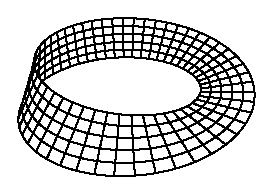
\includegraphics{asy/moebius}
\vskip-0mm
\end{wrapfigure}

One may consider nonoriented surfaces, for example the so called M\"obius strip shown on the diagram.
It turns out that it is possible to generalize Euler's inequality and get an upper for chromatic number for graphs that can be drawn on such surfaces.
(The problem is slightly harder for the so called Klein bottle, but still its difficulty is not comparable with the four color theorem.)

\begin{thm}{Exercise}
Draw the complete graph $K_6$ on a M\"obius strip (assume it is made from a transparent material).
\end{thm}


 
